\section{\textbf{Introduction}}
\IEEEPARstart{W}{e} already stablished that  Finite State Machines (FSM) are widely used as a computation
model in a number of application domains such as data analytics
and data mining \cite{3,4}, network security \cite{5}, bioinformatics \cite{6,7}, tokenization of web pages \cite{9}, computational
finance \cite{9} and software engineering \cite{10}. These applications require processing tens to thousands of patterns for a stream of
input data.\\
\begin{figure}[!h]
    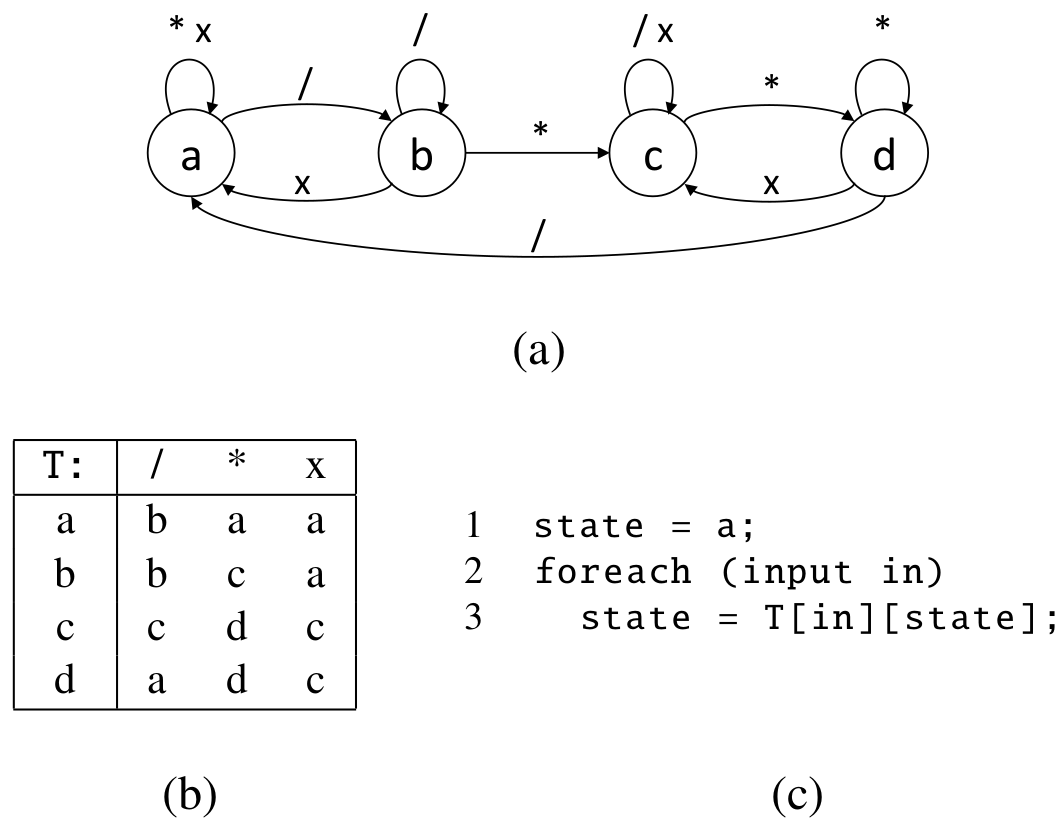
\includegraphics[width=0.50\textwidth]{fsm.png}
    \caption{An FSM containing four states that accepts C style comments in source code delineated by /* and */. The
    input x represents all characters other than / and *. Taken from \cite{2}}
    \centering
\end{figure}
NFAs form the core of many end-to-end applications that utilize pattern matching.
 These pattern matching routines are typically
implemented as if-else or switch-case nests in conventional CPUs
and contribute to a significant fraction of the overall execution time
because of poor branch behavior and irregular memory access patterns.\\
Figure 1(a)  shows an example FSM.
The table in Figure 1(b) determines how the FSM states transition
 on each input symbol, and Figure 1(c) is a straightforward implementation of this FSM that iteratively accesses
the transition table to obtain the state after each input symbol.
FSMs are difficult to parallelize for two reasons. First,
there is a tight dependence between successive loop-iterations
making it nontrivial to distribute loops across multiple
processors. Second, FSMs perform little computation in
each iteration with memory-access patterns that are input-dependent and unpredictable.
This makes it difficult for
FSM implementations to use parallelism within a processor,
namely instruction-level parallelism, vector (SIMD) capabilitiesand memory-level parallelism.
Also the FSM computation, especially Non-Determinstic Finite Automata
(NFA) computation is inherently hard to speedup. Modern multicore
 processors are limited by the number of transitions they can do
per thread in a given cycle, limiting the number of patterns they can
identify. Their processing capability is also limited by the available
memory bandwidth. GPGPUs have limited success with automaton
processing because it is inherently dominated by irregular memory
access patterns. 
n comparison, custom architectures which facilitate in-situ computation in memories can facilitate highly parallel and energy efficient processing of finite state automata in hardware. For instance,
Micron’s Automata Processor (AP) \cite{11} has been shown to accelerate several applications like entity resolution in databases (by
434×) and motif search in biological sequences  (by 201×).
Recent efforts from Virginia’s Center for Automata Processing has
demonstrated that AP can outperform GPGPUs by 32×, and accelerators such as XeonPhi by 62×, across a wide variety of automata
benchmarks .
The Micron AP is a generalized accelerator supporting many application domains which can benefit from fast NFA processing and is
not limited to regular expressions.The success of AP relies on three
factors: massive parallelism, eliminating data movement (between
memory and CPU) overheads, and reducing instruction processing
overheads significantly. Massive parallelism follows from the fact that all state elements (mapped to columns in DRAM arrays) can be
independently activated in a given cycle. An AP chip can support
up to 48K transitions in each cycle. Thus it can efficiently execute
massive Non-deterministic Finite Automata (NFA) that encapsulate
hundreds to thousands of patterns.
The technique we first analyze to perform FSM parallelization is just a logical inference. It says that we have to start by partitioning the input string into segments, and processing these segments concurrently. The problem with this approach is that starting states for each segment are unknown except the first segment (which starts from the FSM’s designated start states). The starting states for a segment are essentially the ending states of the previous segment.The work \cite{2} has solved this by executing the input segment for every
state of the FSM by leveraging classic parallel prefix-sum . This
method is referred to as enumerative computation as it enumerates
all possible start states. We refer to the sequence of states visited by
each enumeration start state as the enumeration path. Once the first
segment is finished, we know the correct start states of the second
segment and can pick the results of enumerated paths belonging to
the correct start states (Figure 3 discuss an example
enumeration).\\
While enumerative approach is promising, there were several challenges to realize it in AP. In a conventional processor a SIMD thread
can process enumeration paths and thread’s local variables keep
track of the start state for each enumerated path. Tracking the start
state of an enumerated path is important for combining the results of
individual input segments as discussed above. In the AP, there is no
notion of software threads or local variables which can keep track
of start states of enumerated paths. A processing unit or half core
simply accepts a stream of input symbols and does transitions via
a routing matrix (custom interconnect) each cycle. Thus it can be
challenging to execute concurrently and keep track of all enumeration paths. Another critical challenge to be solved is taming the
enormous computational complexity of enumeration. Enumerations
can be highly inefficient because in the worst case each state has
to be enumerated. NFAs can have several thousands of states.\\
The architecture that \cite{1} provides, solves the above problems by leveraging some unique properties of NFAs and unique features of the AP. For instance, we utilize the connected components (disconnected subgraphs) in an NFA to merge enumeration paths and thereby take
advantage of the massive parallelism of the AP. Furthermore, the
range (or all reachable states) of an input symbol can be utilized to
prune the enumeration paths. Another NFA property we leverage is
based on parent states in an NFA. If the start states of enumeration paths have a common parent state, they can be merged. Similar to
the work of  \cite{2}, we observe enumeration paths converge at run time and implement dynamic convergence checks in AP. To solve the
start state tracking problem, we utilize AP flows. The flow abstraction also allows for near-zero overhead convergence checks. Our
framework also discusses the details of combining the results from
input segments, and hiding these processing overheads by leveraging
the asymmetric finish times of input segments.\\
In summary this review offers the following analysis:
\begin{itemize}
    \item Parallelization of non deterministic FSMs on the Automata Processor (AP).
    \item Explore the challenges in parallelizing FSMs in AP.
    \item Quick look to evaluation of the technique against benchmarks.
    
\end{itemize}

